%================================================
%	PACKAGES AND THEMES
%================================================
\documentclass[t,aspectratio=169,xcolor=dvipsnames]{beamer}

\usetheme{SimplePlusAIC}

\usepackage{hyperref}
\usepackage{graphicx} % Allows including images
\usepackage{booktabs} % Allows the use of \toprule, \midrule and  \bottomrule in tables
\usepackage{svg} % Allows using svg figures
%\usepackage{makecell}
\newcommand*{\defeq}{\stackrel{\text{def}}{=}}
\usepackage{setspace}
\usepackage[T1]{fontenc}
\usepackage{helvet}
%\usepackage{textgreek}
\usepackage{amsmath}
\usepackage{bm}
\usepackage{ragged2e}
\usepackage{xfrac}
% \usepackage[nice]{nicefrac}
\usepackage[loose]{units}
%\usepackage{braket}
%\usepackage{gensymb}
% \usepackage[cm]{sfmath}
%\usepackage{verbatim}
%\usepackage{fancyvrb}
\usepackage{tikz} % Allows nice main page with logo

%\setbeamertemplate{blocks}[rounded][shadow] % block options

\usepackage[svgnames,table]{xcolor}
\arrayrulecolor{black}
\setlength{\arrayrulewidth}{0.20mm}
\renewcommand{\arraystretch}{1.40}  % stretch tables row size

%================================================
%	TITLE PAGE
%================================================
\title[short title]{Le chapitre français du CAA} 
\subtitle{\textit{Computer Applications and Quantitative Methods in Archaeology} -- CAA-FR}

\author{https://caafrance.hypotheses.org}
% \institute[CBI]{Center for Anything, Department of Something \\ University of Anywhere \\ Somewhere \\ ~ \\}

\date{\textcolor{nyublue}{GMPCA 2025, Rouen, 14 avril 2025}}

%================================================
%	BEGIN DOCUMENT 
%================================================
\begin{document}

%------------------------------------------------
%	TITLE SLIDE
%------------------------------------------------
\begin{frame}[plain]

    \titlepage
    
\end{frame}

%------------------------------------------------
%	NEW SLIDE
%------------------------------------------------
\begin{frame}{overview caa-int}

    \frametitle{CAA International} 
    %\framesubtitle{National Chapters of the CAA-Int.}

    %\vspace{0.5mm}

    \begin{figure}
        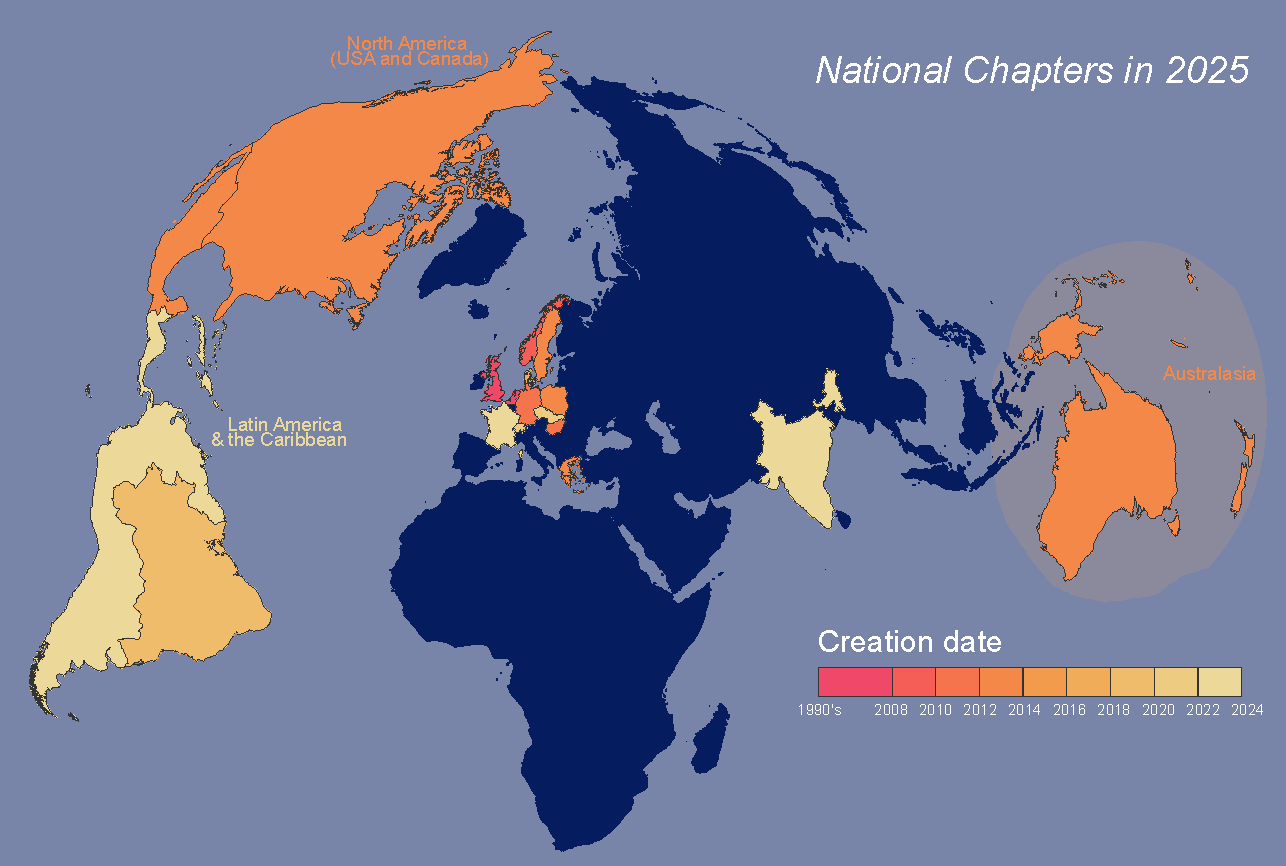
\includegraphics[height=0.92\textheight]{figures/national-chapters2025.pdf}
    \end{figure}

\end{frame}

%------------------------------------------------
%	NEW SLIDE
%------------------------------------------------

\begin{frame}{overview caa-fr 1}

    \frametitle{Overview of the CAA-FR} 
    %\framesubtitle{Overview}

    % \vspace{-2mm}

    \begin{block}{\textbf{Creation and Objectives}} % block is purple, alertblock orange and exampleblock in blue-green
       
        \begin{itemize}
            \item \textbf{2024}: Creation during CAA Conference in Auckland
            \item To bring together archaeologists, archaeometrists, mathematicians, computer scientists and members of other disciplines based in France to complement and extend the interests of CAA International
            \item To encourage communication between these disciplines
            \item To give a survey of present work in the field
            \item To stimulate discussion and future progress in the application of information technology to archaeological research and practice
            \item To provide guidance and support in the form of seminars and/or workshops
        \end{itemize}

    \end{block}

    \end{frame}

    \begin{frame}{overview caa-fr 2}

    \frametitle{Overview of the CAA-FR} 
    %\framesubtitle{Overview}
        \begin{block}{\textbf{Current \textit{Bureau}}}
       
        \begin{itemize}
            \item \textbf{2024-2025} \& an election biennially at the CAA-FR General Meeting
            \item \textbf{Three speakers}: Dr Nicolas Frerebeau (UMR 6034 Archéosciences Bordeaux), Dr Sébastien Plutniak (UMR 7324 CITERES), Dr Gwénaëlle Moreau (SpaceARC).% j'ai fait du copier-coller, si ça tient à moi > je virerai le "Dr"
            \item \textbf{Three vice-speakers}: Dr Anaïs Vignoles (MSCA fellow), Mathias Bellat (PhD candidate, University of Tübingen), Dr Julie Gravier (UMR 6049 ThéMA)
        \end{itemize}

    \end{block}
    
    \end{frame}

%------------------------------------------------
%	NEW SLIDE
%------------------------------------------------
\begin{frame}{colloque ACQuA}

    \frametitle{Activities since 2024} 
    %\framesubtitle{Subtitle}

    \begin{block}{\textbf{ACQuA Colloquium (Jan. 2025)}}
    	\begin{itemize}
    		\item https://acqua.sciencesconf.org/
    	\end{itemize}
    \end{block}
    
    %\vspace{4mm}
    
    \begin{columns}[t]
    	
    	\column{0.5\textwidth}
    	
    	\begin{figure}
    		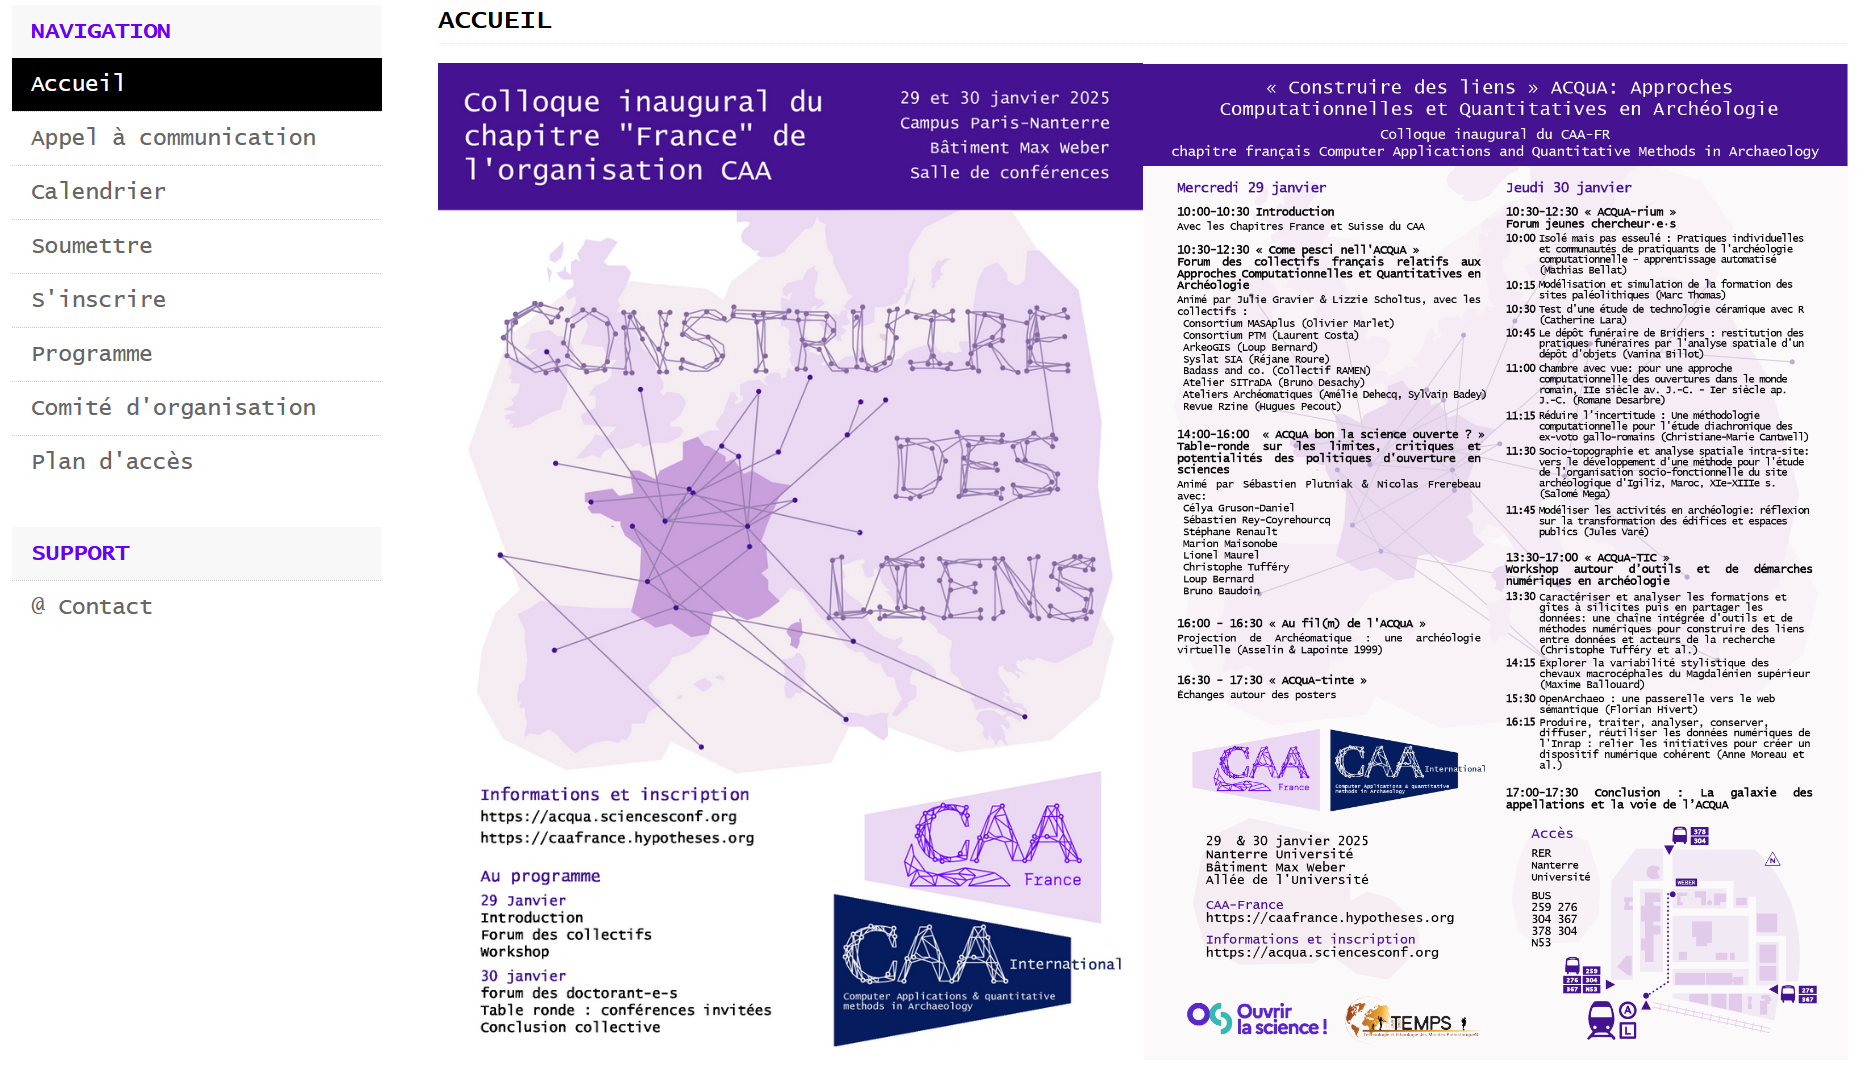
\includegraphics[height=0.48\textheight]{figures/acqua2025.png}
    	\end{figure}
    	
    	\column{0.5\textwidth}
    	
    	\textbf{4 formats}
    	
    	\begin{itemize}
    		\item Forum of French collectives % Forum des collectifs français : 8 collectifs
    		\item Round table on the limits, criticisms and potential of open sciences policies % Table-ronde sur les limites, critiques et potentialités des politiques d'ouverture en sciences > 8 invités
    		\item Forum of young researchers % Forum des jeunes chercheur·e·s présentations flashs > 8 présentations
    		\item Workshop on digital tools and approaches in archaeology % Workshop autour d'outils et de démarches numériques en archéologie > 4 présentations plus longues avec envoi de textes préalablement au workshop
    	\end{itemize}
    	
    \end{columns}
  
\end{frame}

%------------------------------------------------
%	NEW SLIDE
%------------------------------------------------

\begin{frame}{activities}

    \frametitle{Activities since 2024}

    \begin{block}{\textbf{Support for young researchers for CAA Athens 2025}}
       
        \begin{itemize}
            \item In collaboration with the École française d'Athènes
            \item 5 rooms available during the week of the conference % 5 candidatures
        \end{itemize}

    \end{block}

\end{frame}

%================================================
%	END DOCUMENT 
%================================================
\end{document}
